
\subsection{SHMR}
The SHMR for all the galaxies, as well as only the central galaxies, with $M_{*} > 10^8 M_{\odot}$ from TNG is plotted in figure \ref{shmr_res}, along with the best fits from \cite{Moster2012} and \cite{Behroozi2013}.


\begin{figure}
    \centering
    \makebox[\textwidth][c]{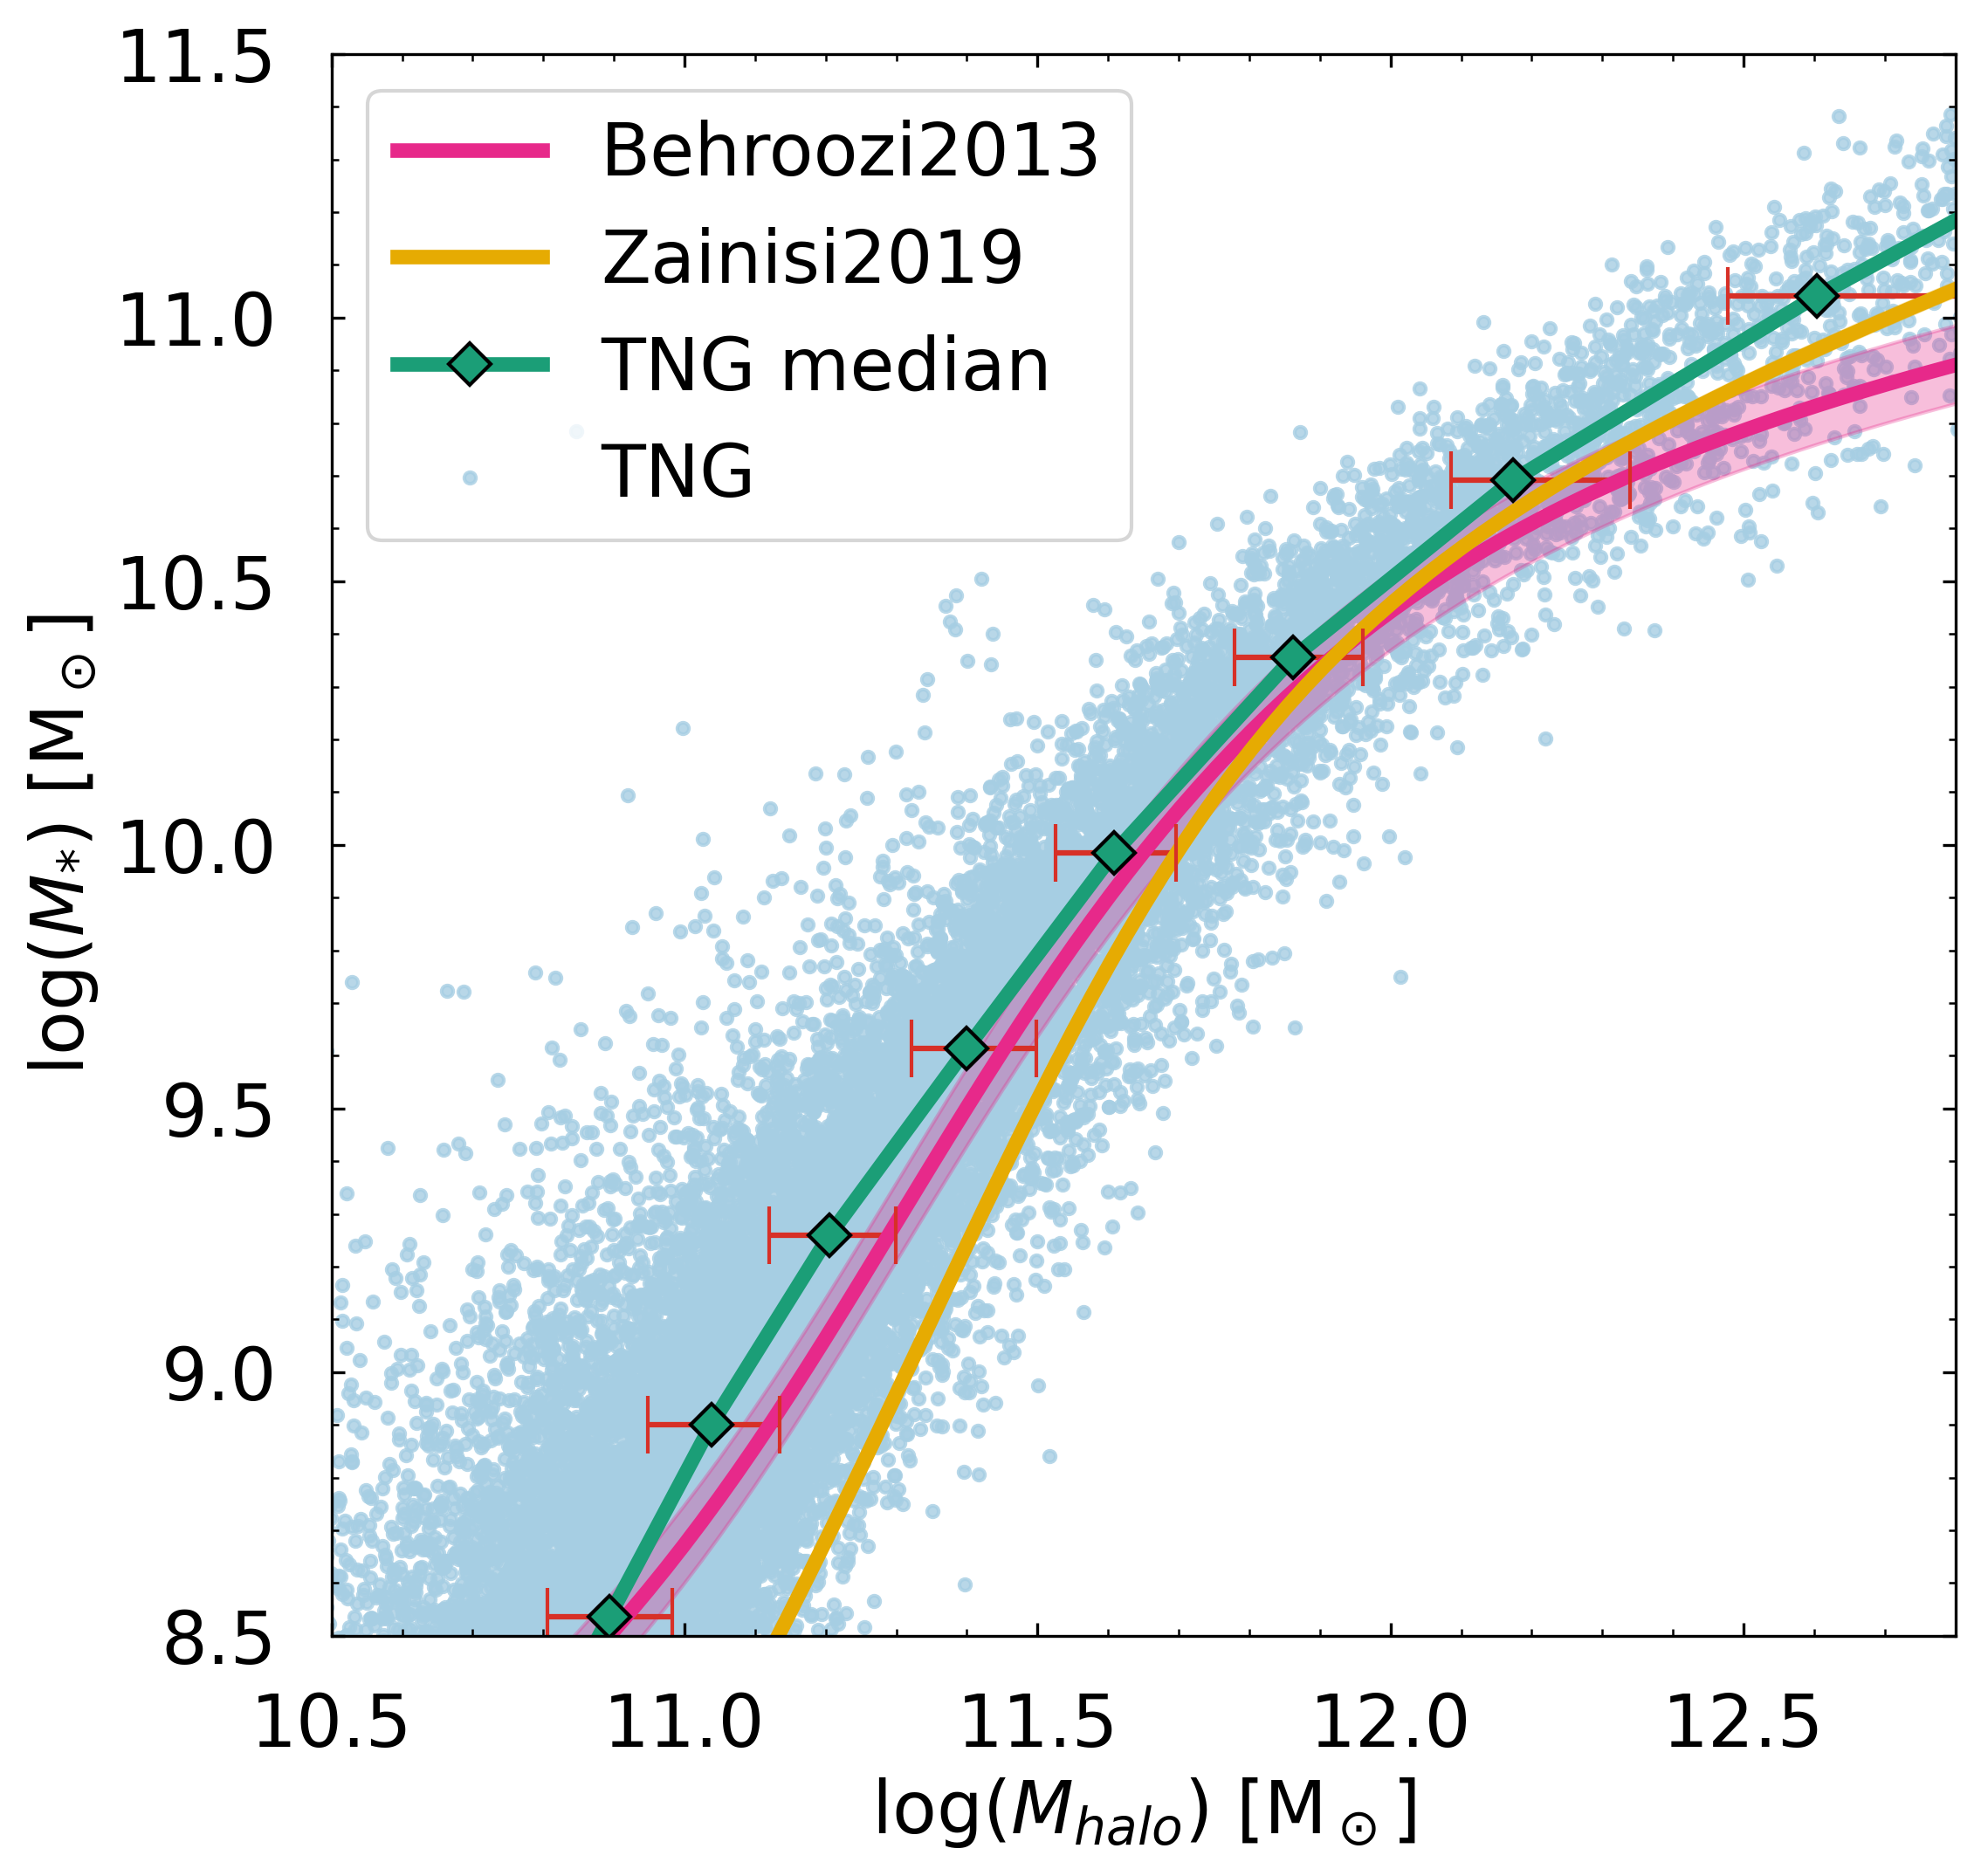
\includegraphics[width=0.9\paperwidth]{images/results_shmr.png}}
    \caption{}
    \label{shmr_res}
\end{figure}


\subsection{TFR}
The TFR for the late type galaxies in TNG100 is shown in Figure \ref{tfr_res}. 

\begin{figure}
    \centering
    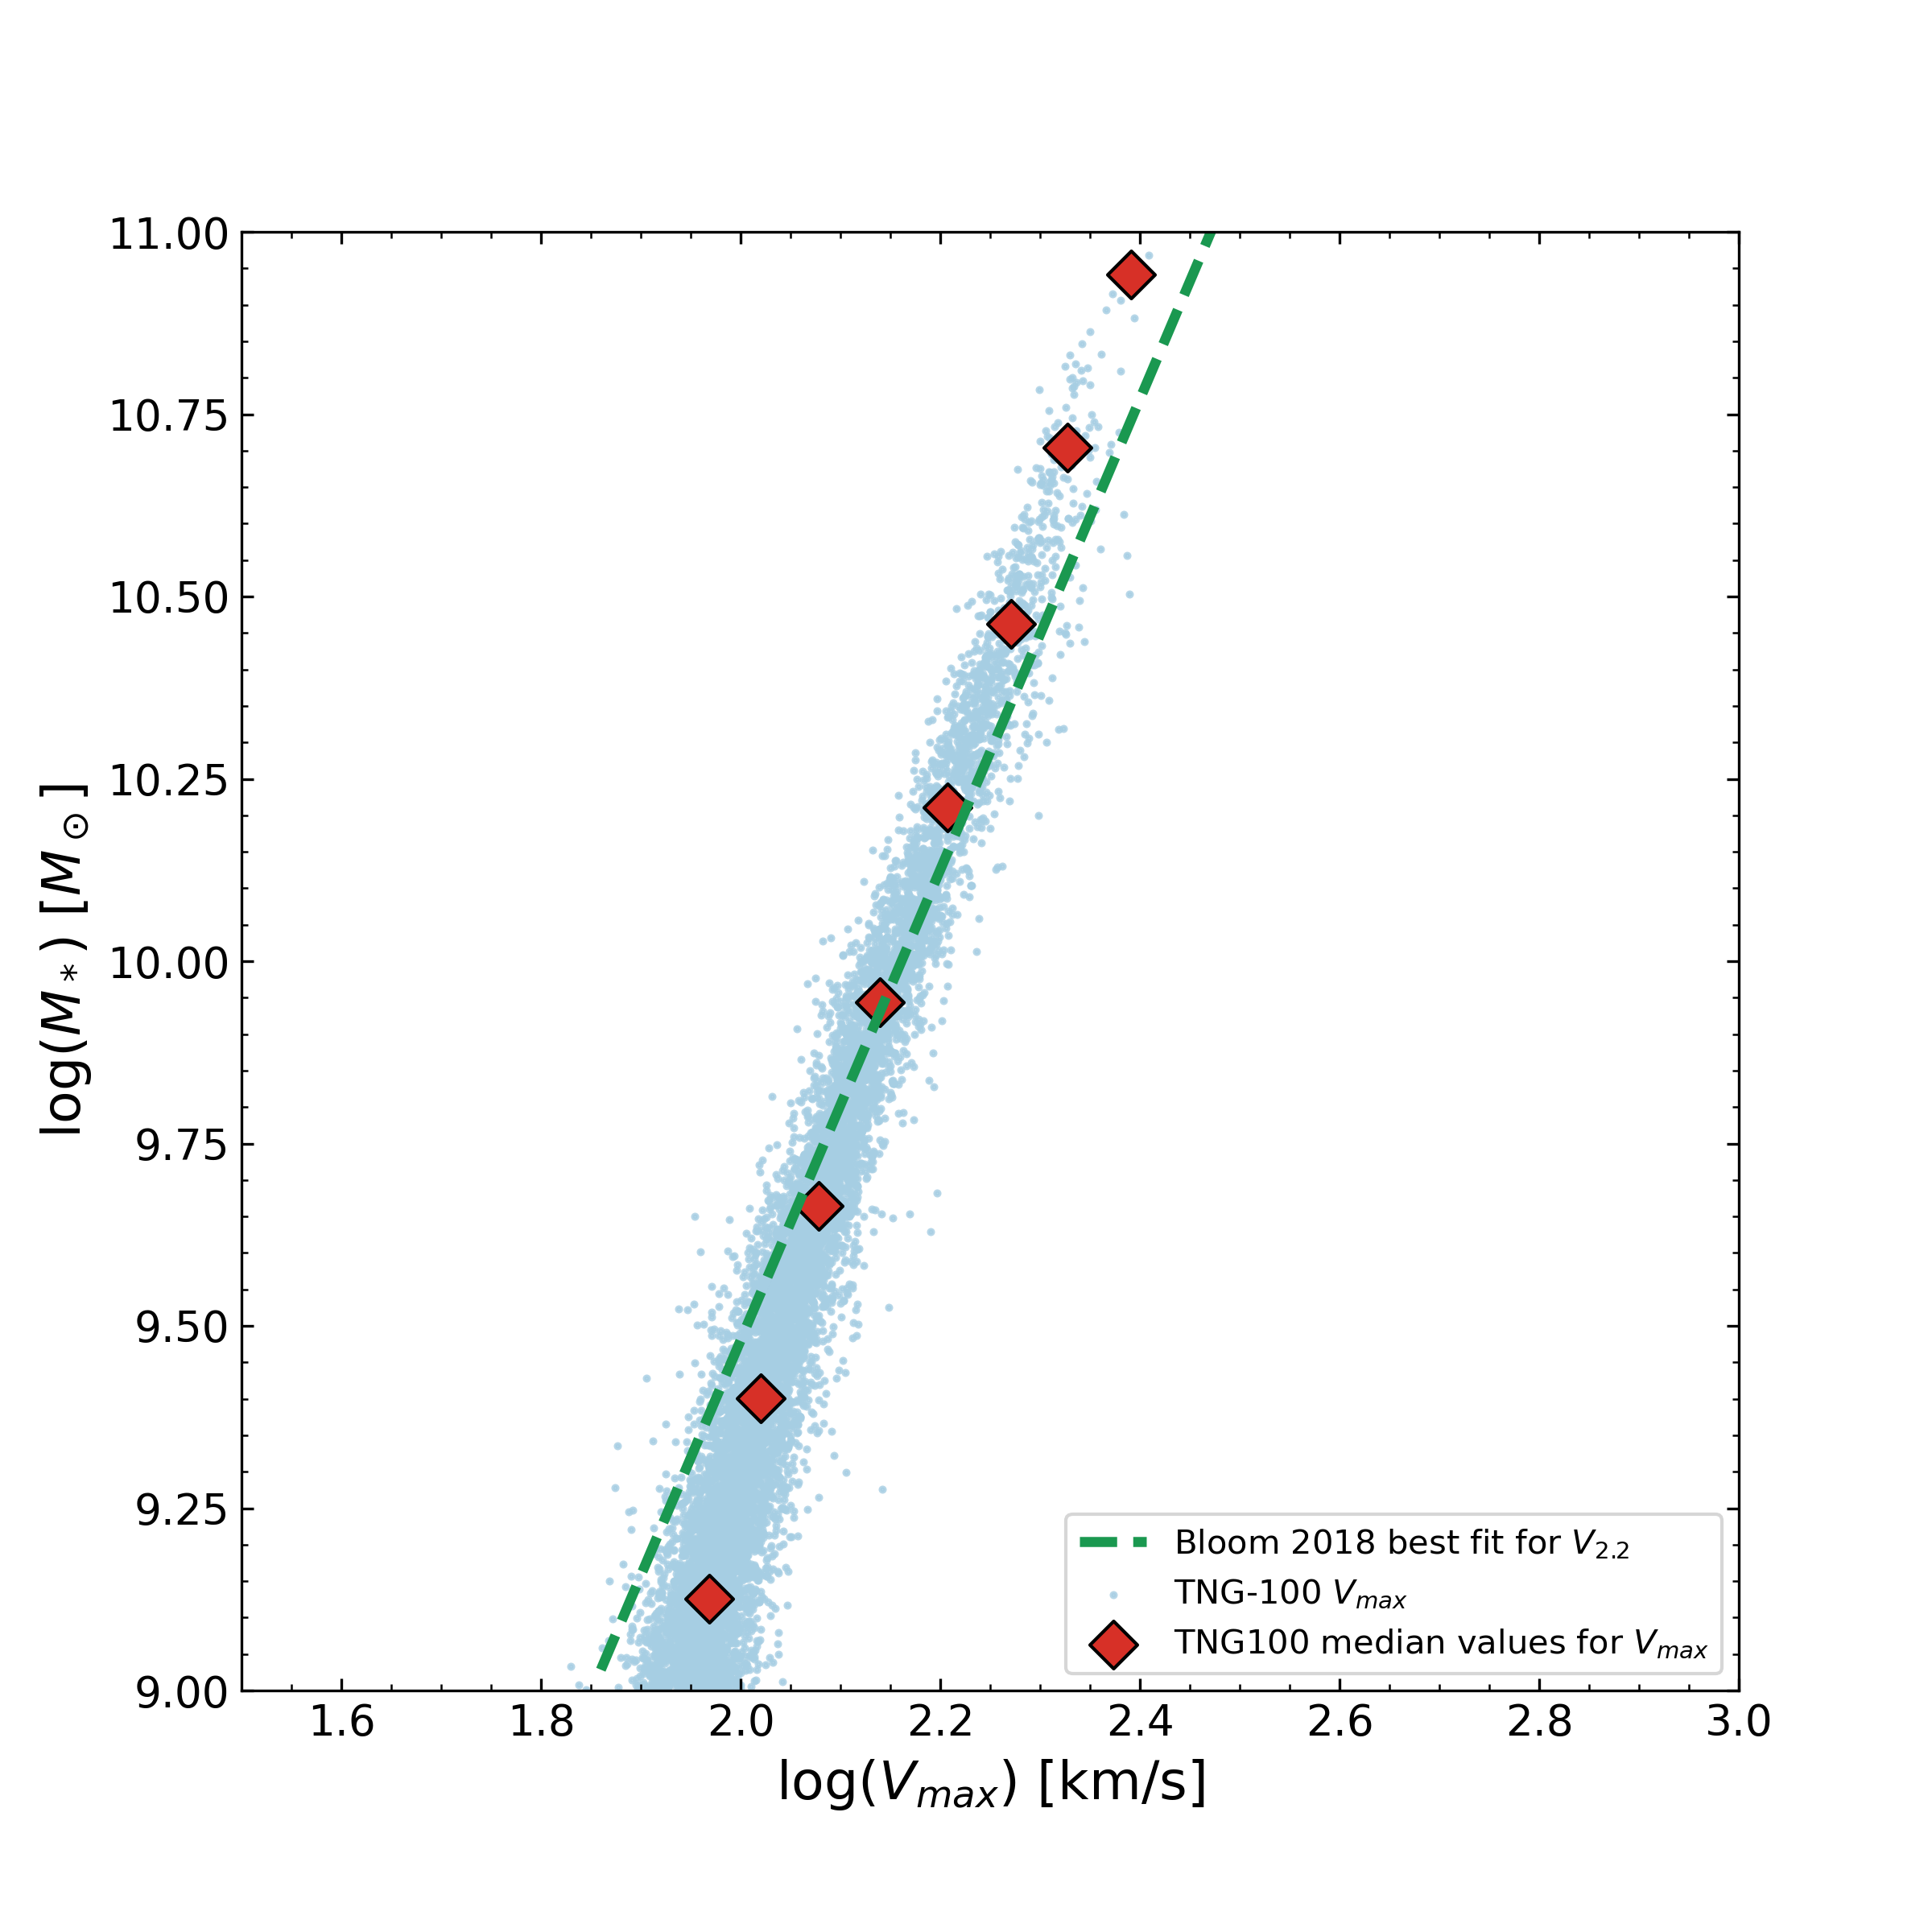
\includegraphics[width=0.9\textwidth]{images/results_tully_fisher.png}
    \caption{}
    \label{tfr_res}
\end{figure}

\subsection{FJ relation and the FP}

The velocity dispersion as function of stellar mass can be seen in Figure \ref{FJ_res}. The trend for the TNG-100 data is a clear power law as expected from the FJ relation. Compared to the observational data, the simulation data shows lower $\sigma$ values, by about 0.1-0.2 dex. This could be explained by the fact that the $\sigma$ in the TNG galaxies is averaged across all particles, across the whole size of the subhalo. In general, gas has a lower $\sigma$ than stars and dark matter, so this could push the total $\sigma$ down. However, in early-type galaxies there is little gas so the impact would be expected to be small. The fact that $\sigma$ is found by averaging across the entire subhalo would include particles further out than for the SAMI data in which the velocity dispersion is averaged inside the effective radius ($\sigma_{e}$) is used. Other studies have also found that simulations tend to get lower values for $\sigma$ \parencite{Sande2018}, so this might also just be a limitation of the simulations.

The other relations in the fundamental plane are shown in Figures \ref{FP_res1} and \ref{FP_res1}.

\begin{figure}
    \centering
    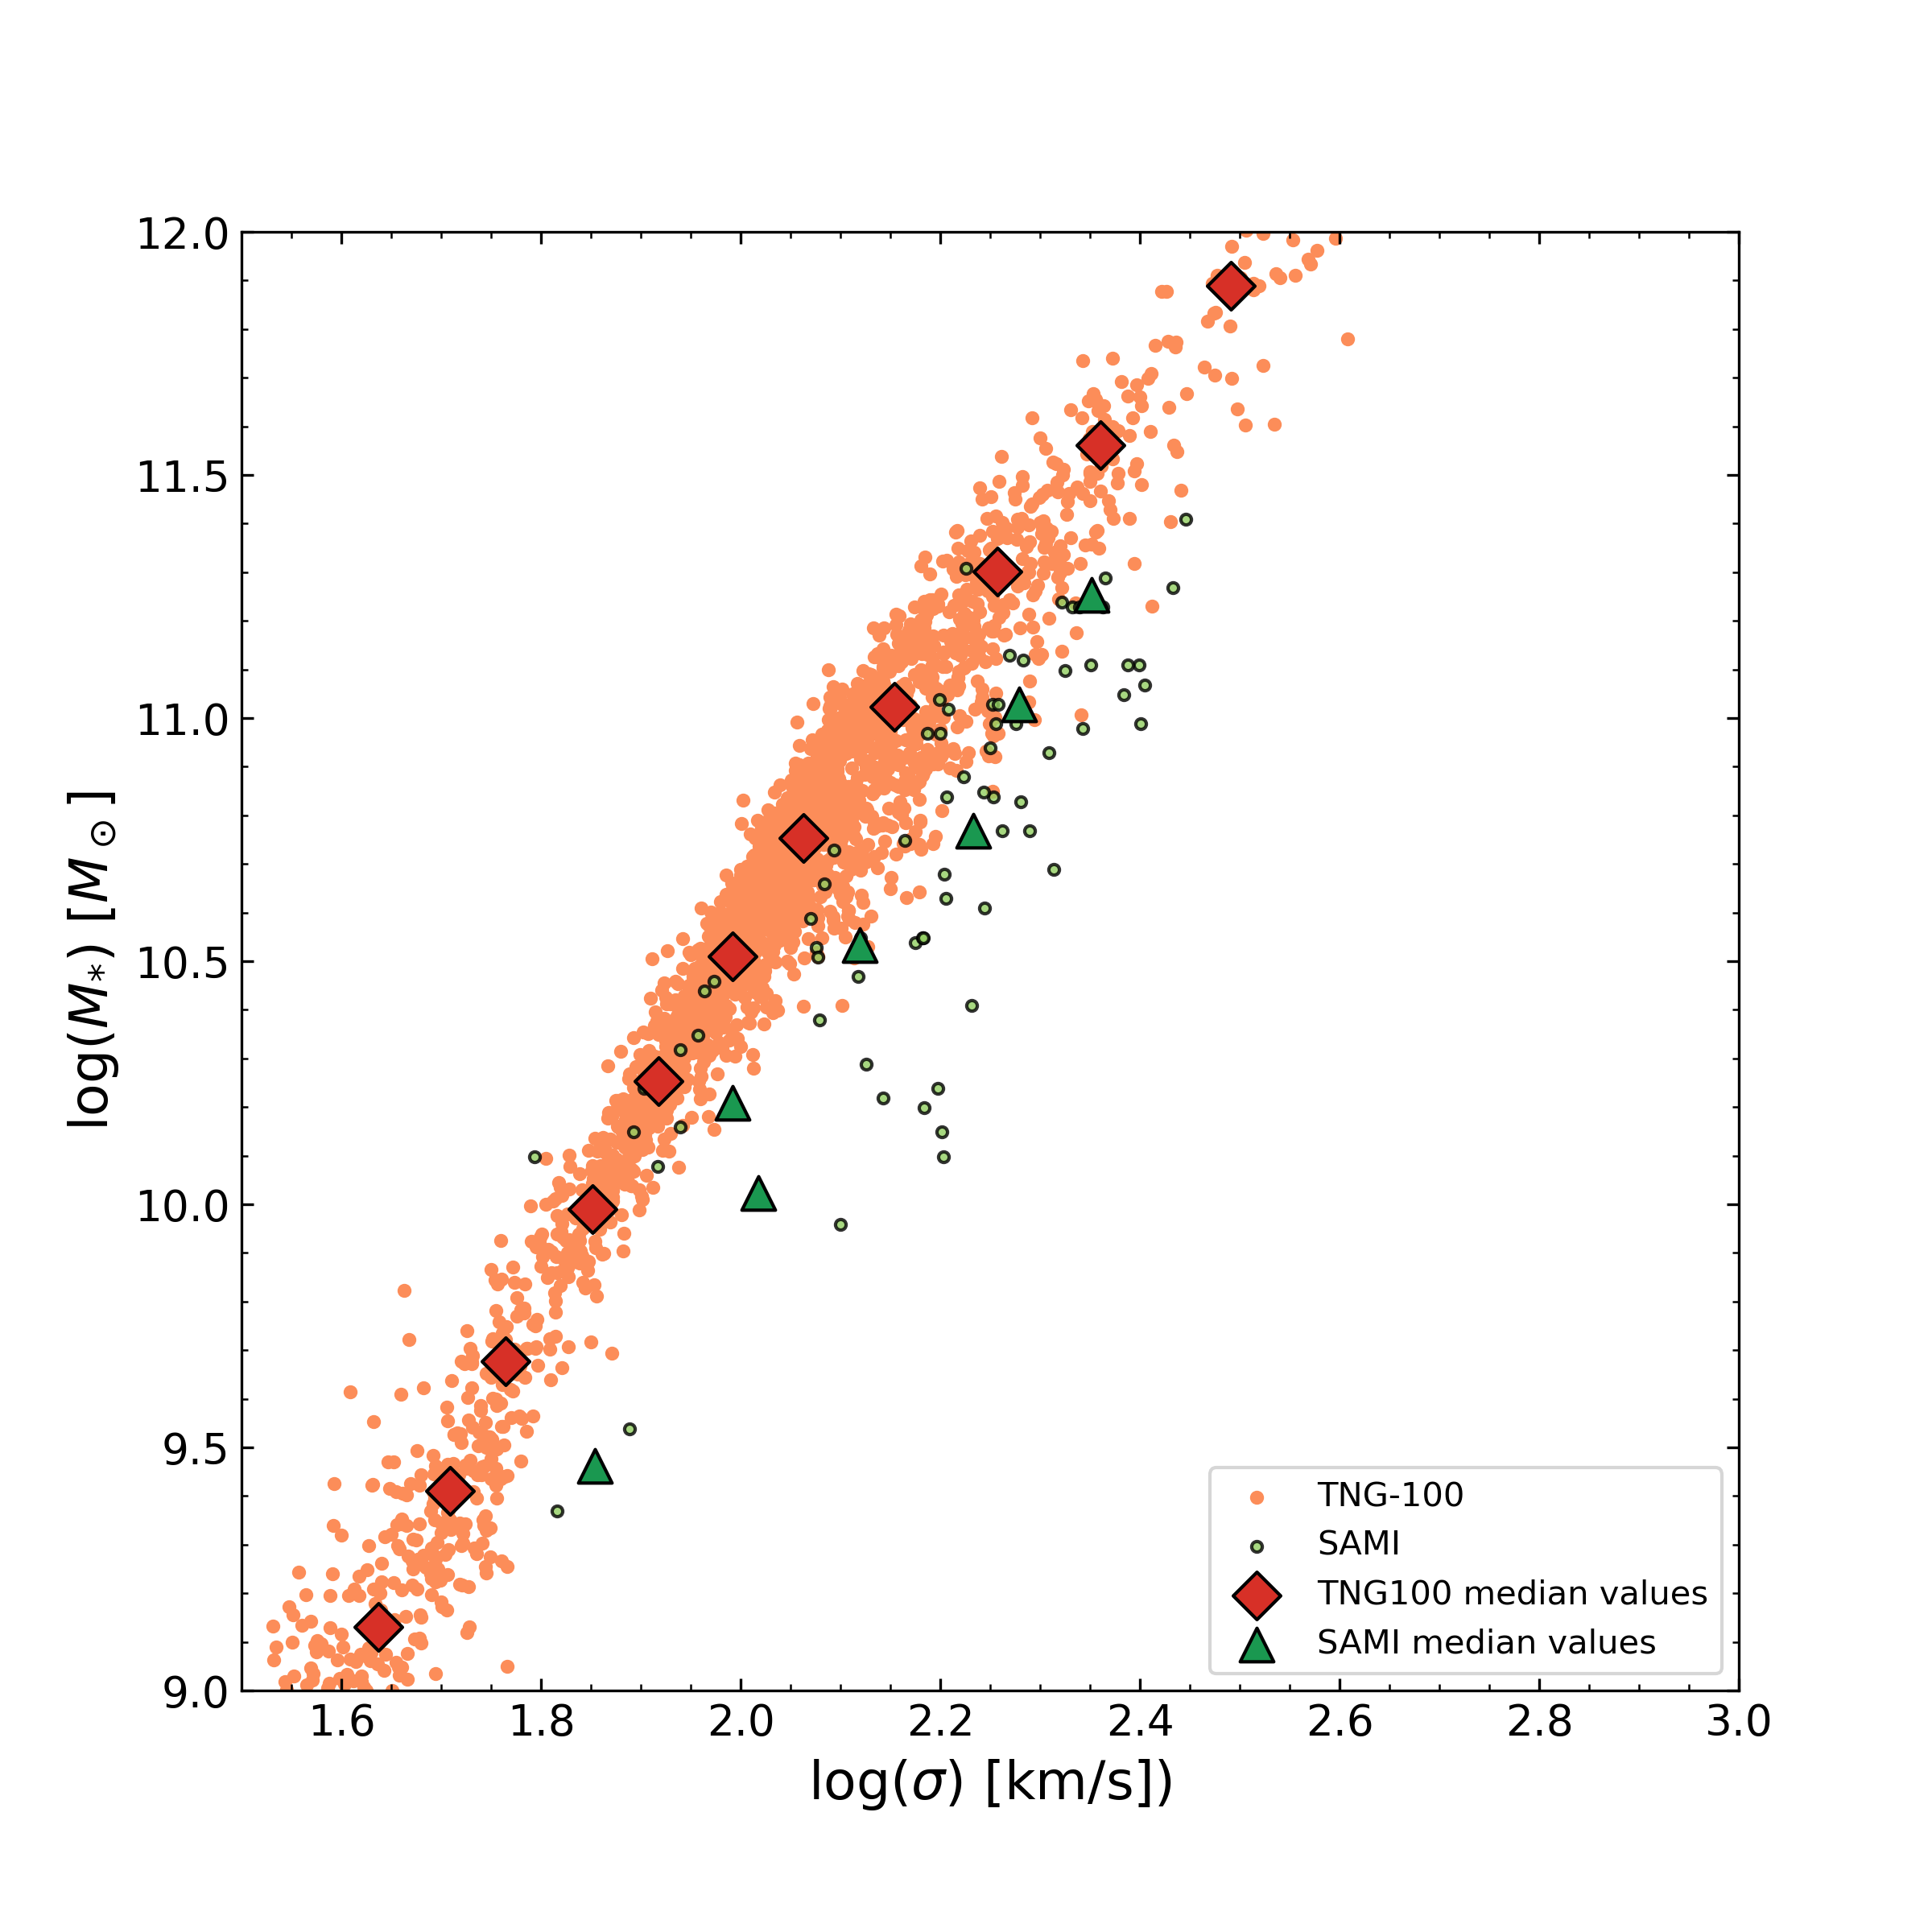
\includegraphics[width=\textwidth]{images/results_faber_jackson.png}
    \caption{Early type galaxies for both TNG and SAMI.}
    \label{FJ_res}
\end{figure}

\begin{figure}
    \centering
    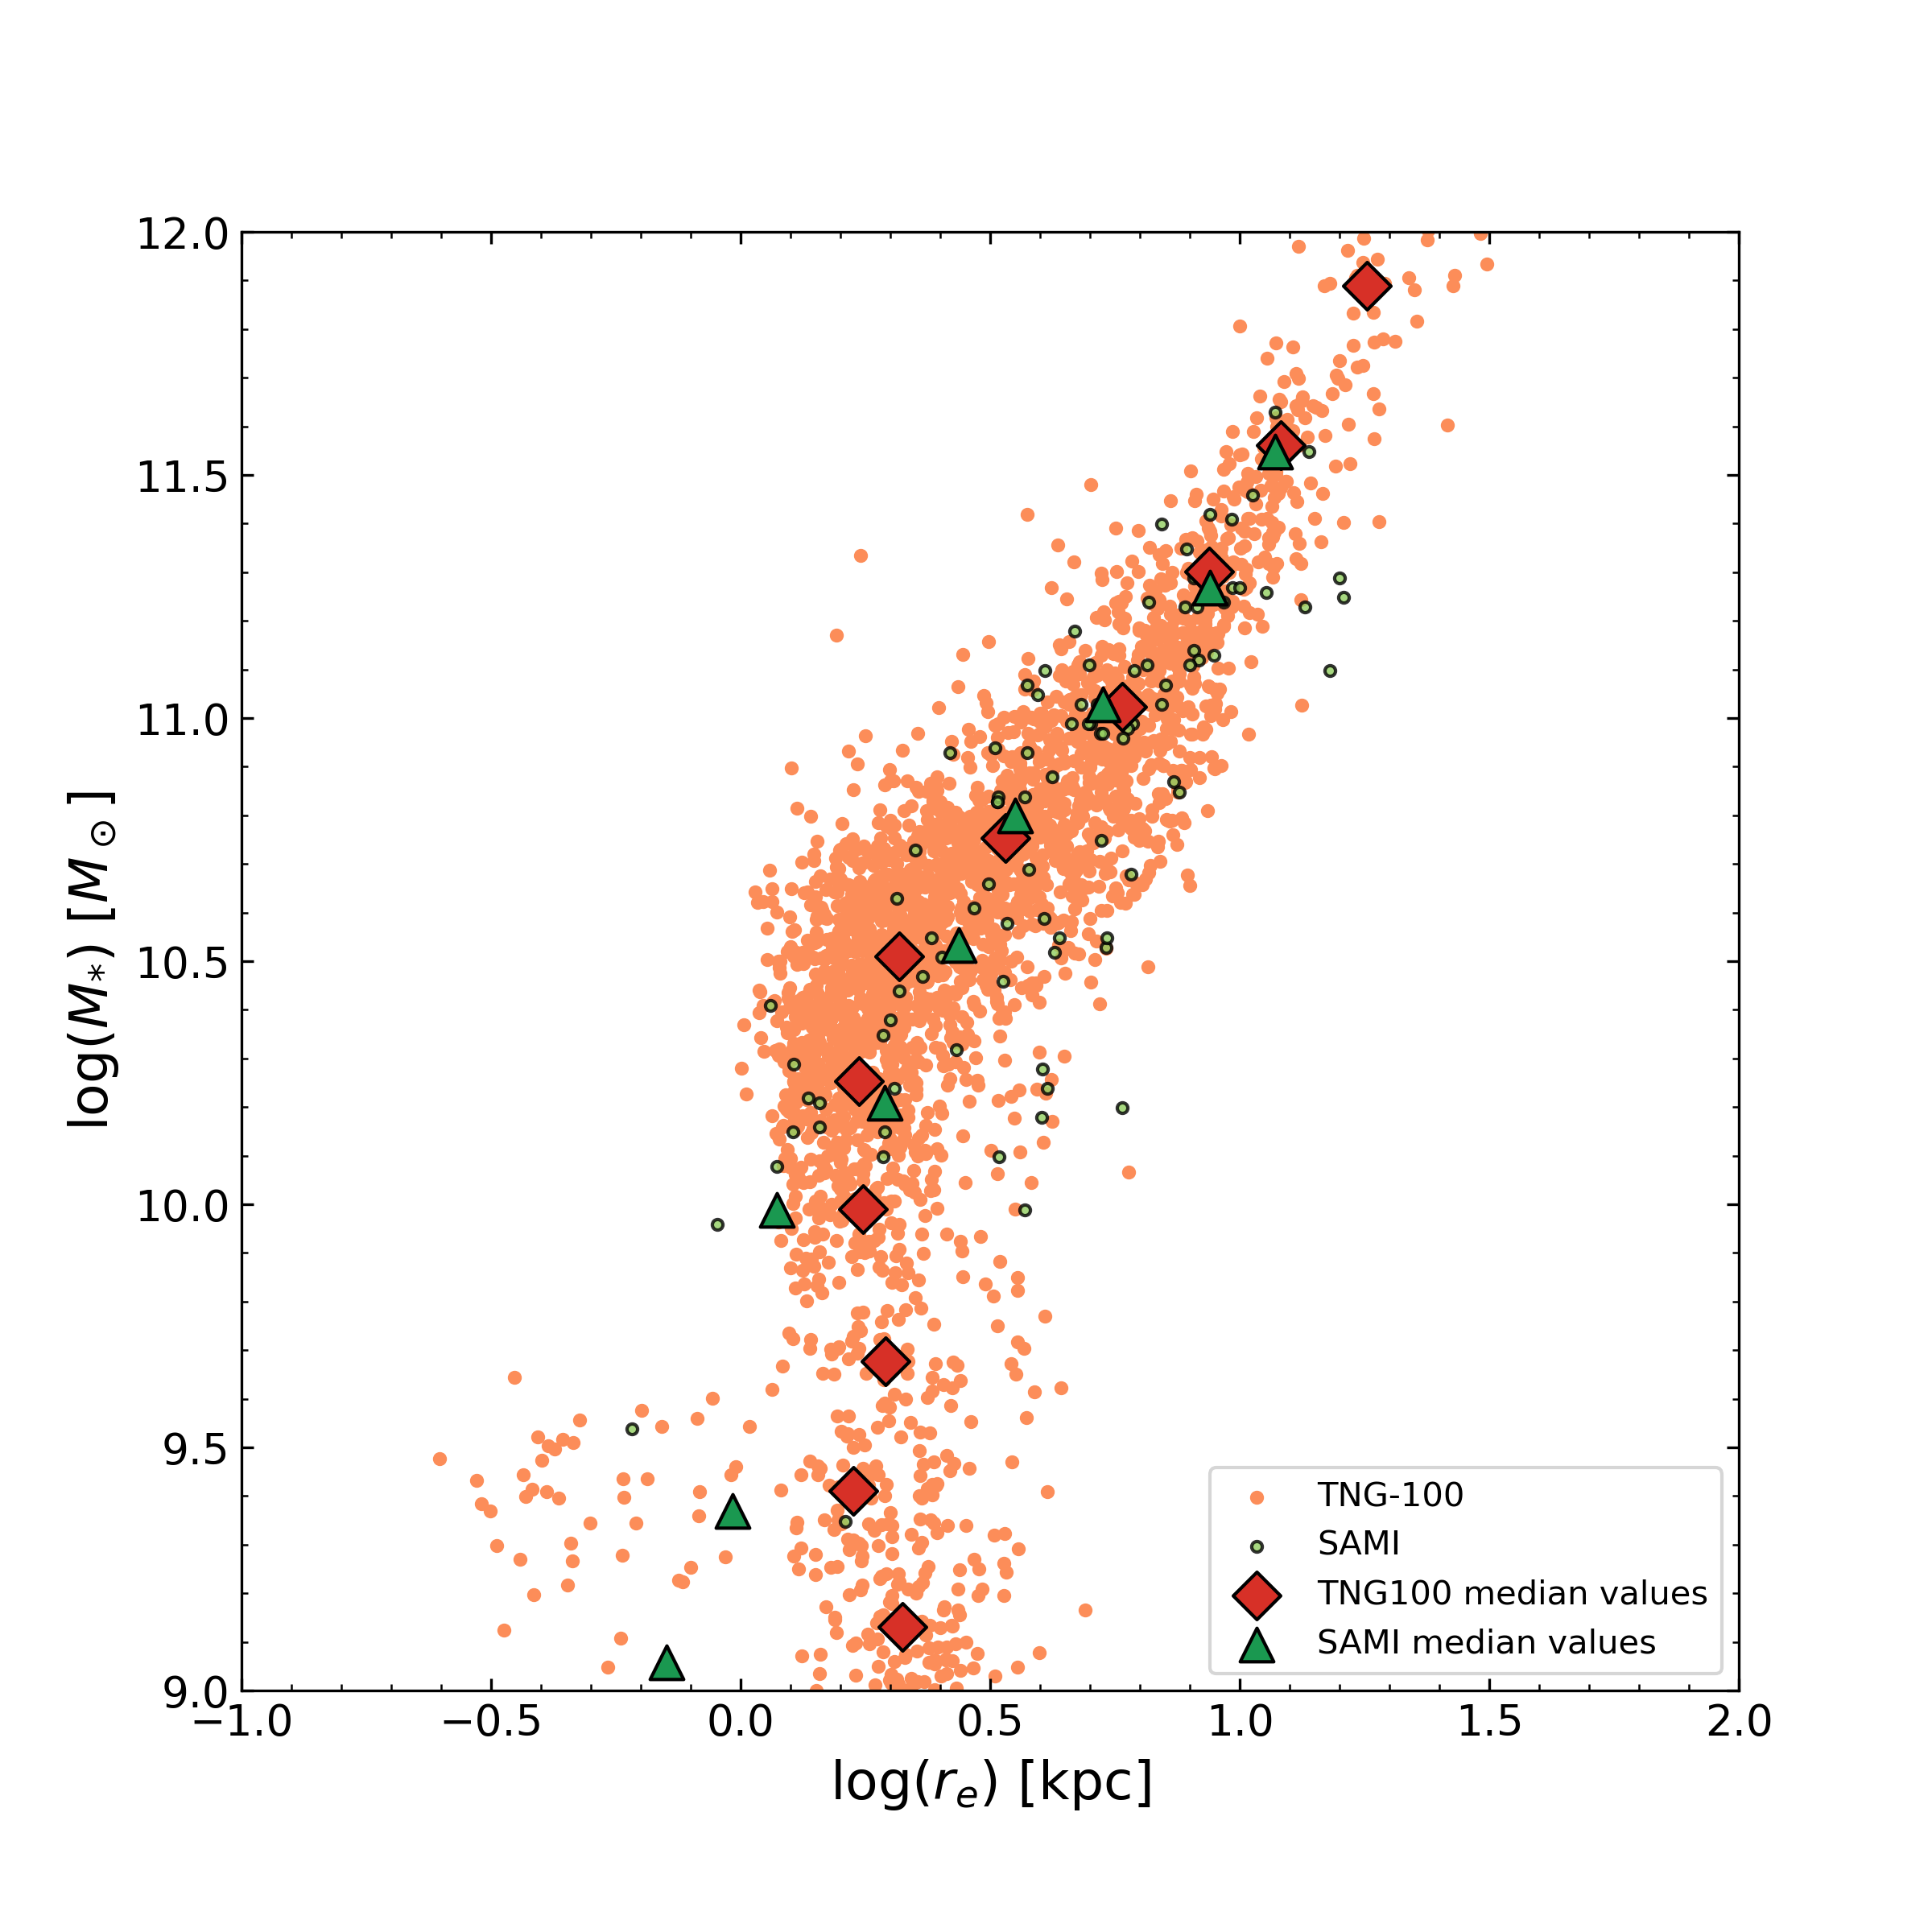
\includegraphics[width=\textwidth]{images/results_mass_radius_FP.png}
    \caption{Early type galaxies for both TNG and SAMI.}
    \label{FP_res1}
\end{figure}

\begin{figure}
    \centering
    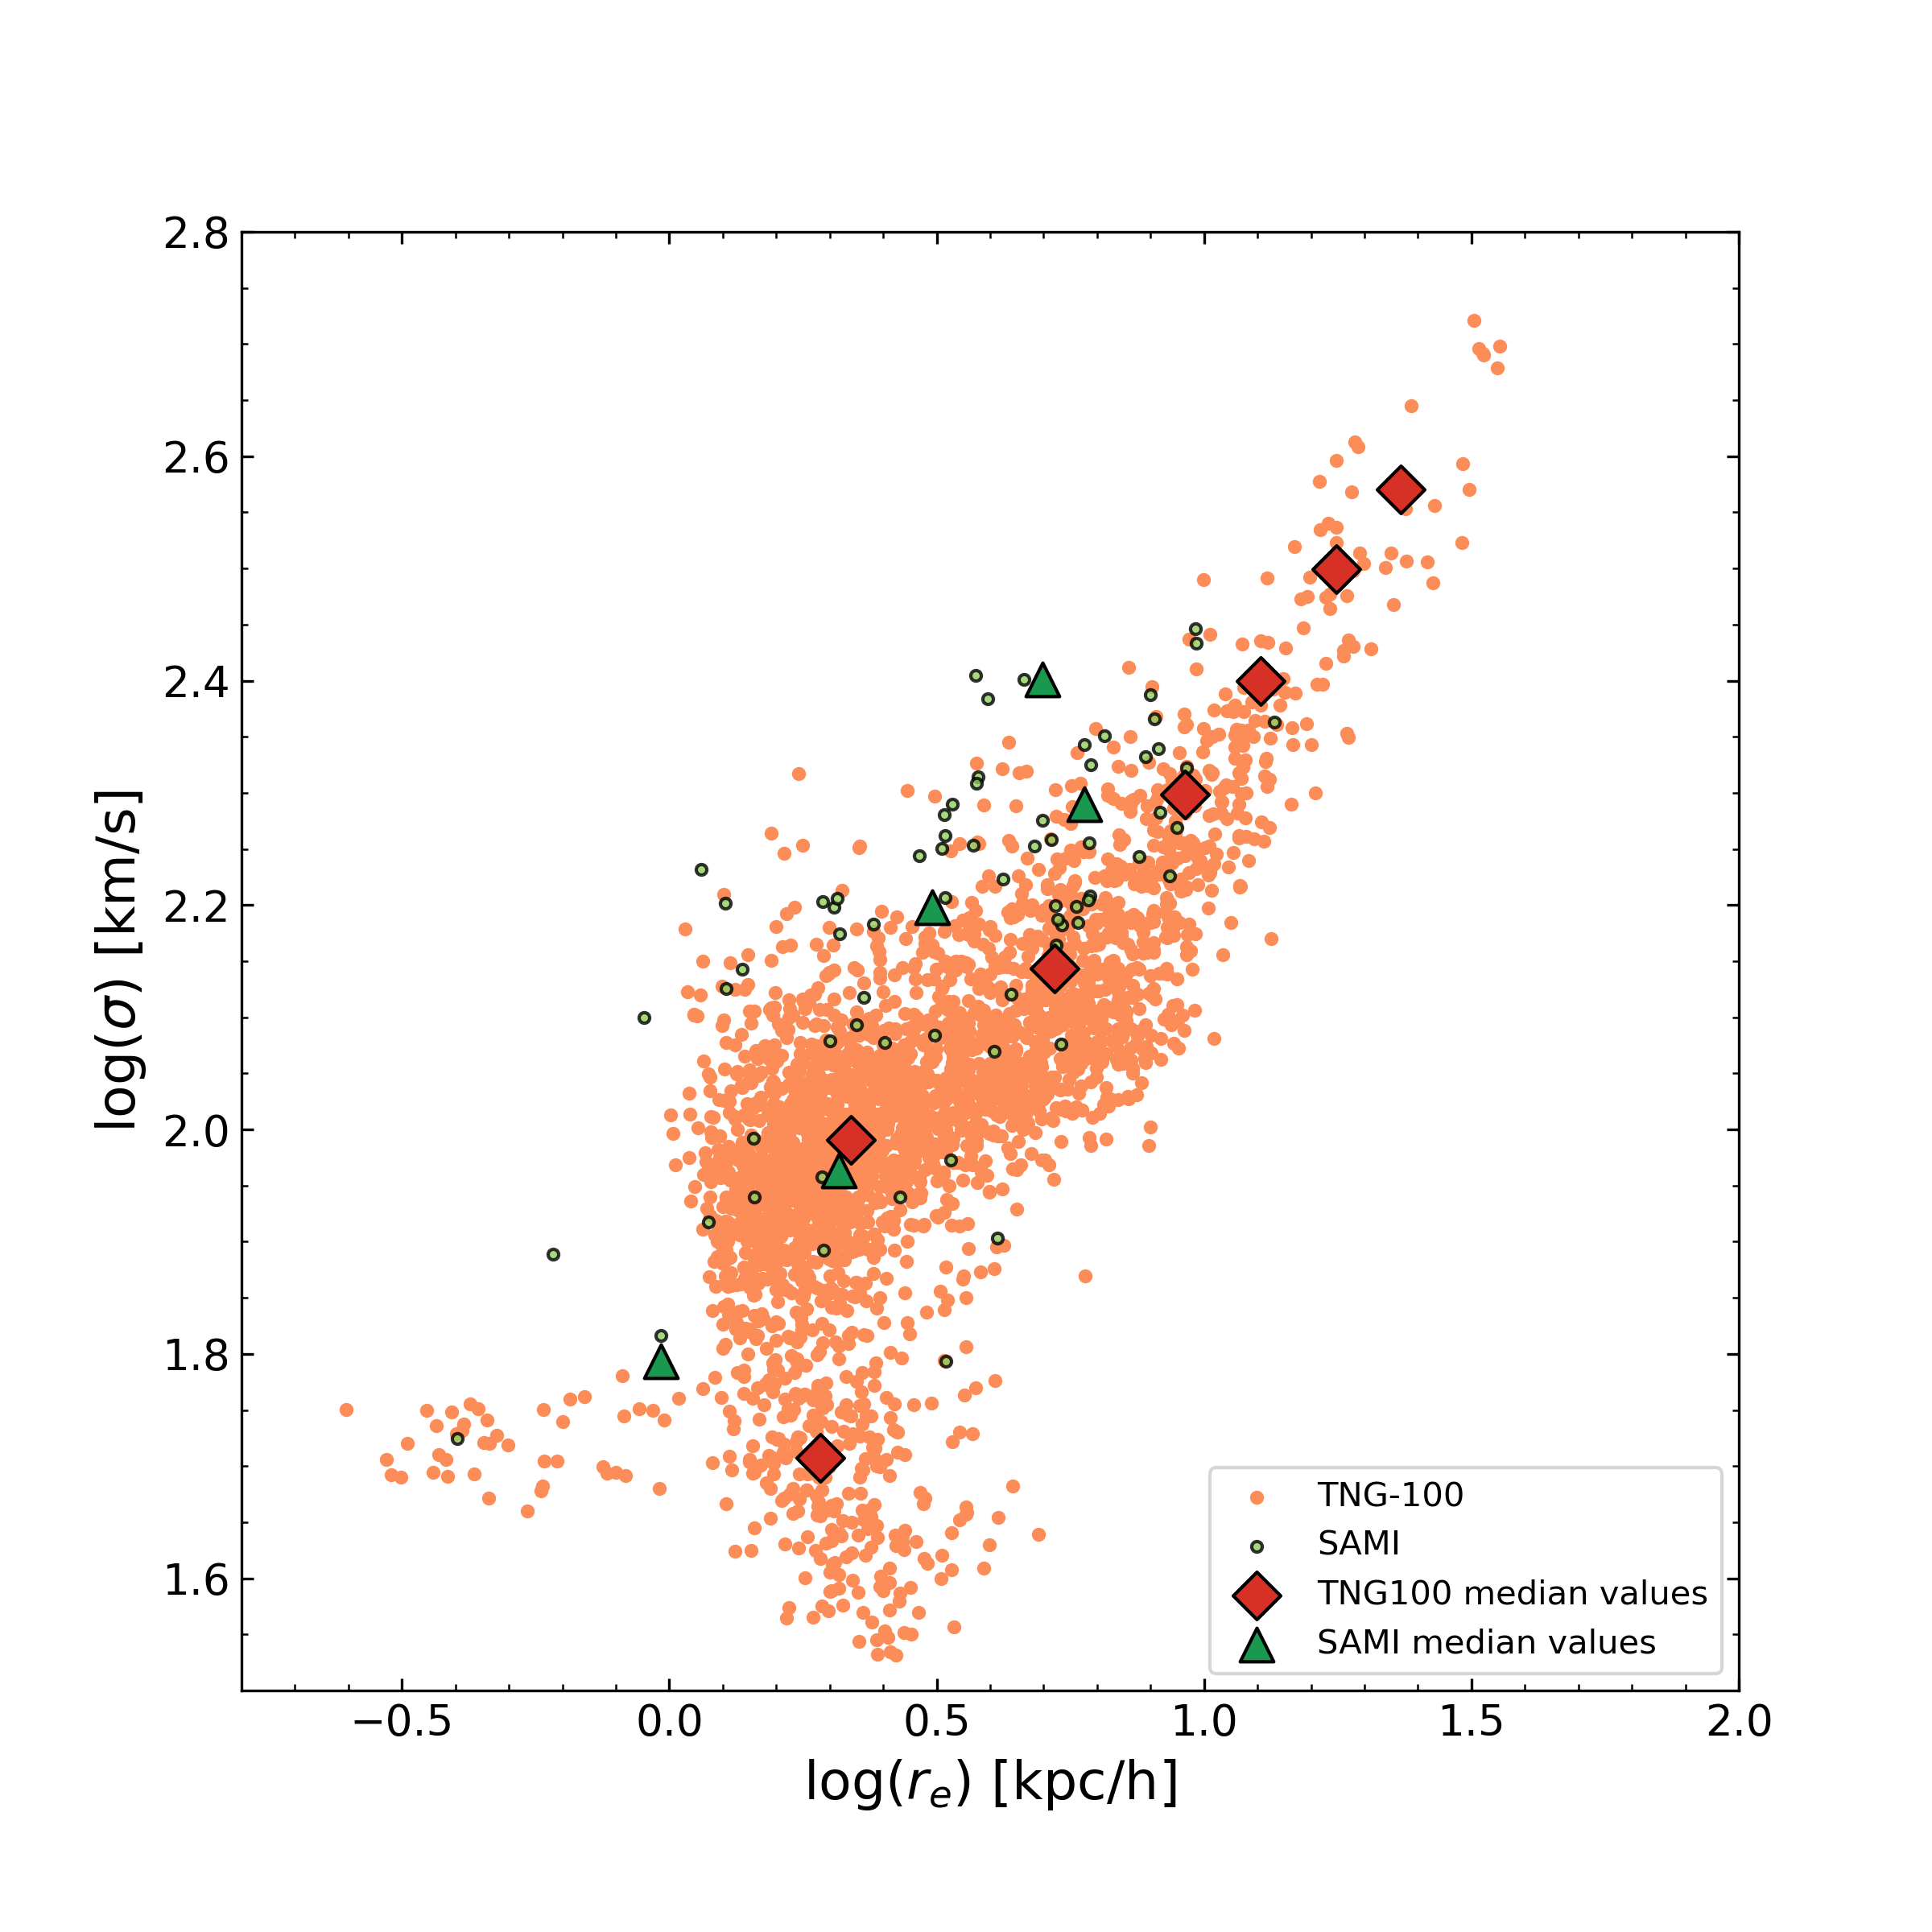
\includegraphics[width=\textwidth]{images/results_sigma_radius_FP.png}
    \caption{Early type galaxies for both TNG and SAMI.}
    \label{FP_res2}
\end{figure}

\subsection{Color bimodality}
The color mangitude diagrams for different filters are shown in Figure \ref{color_magnitude_res}.

Figure \ref{pdf_color_res1} shows the probability density function (PDF) for TNG100 early and late type galaxies. In Figure \ref{pdf_color_res2} the PDF for the TNG100 g-r band and the SAMI g-r band are shown.

\begin{figure}
    \centering
    \makebox[\textwidth][c]{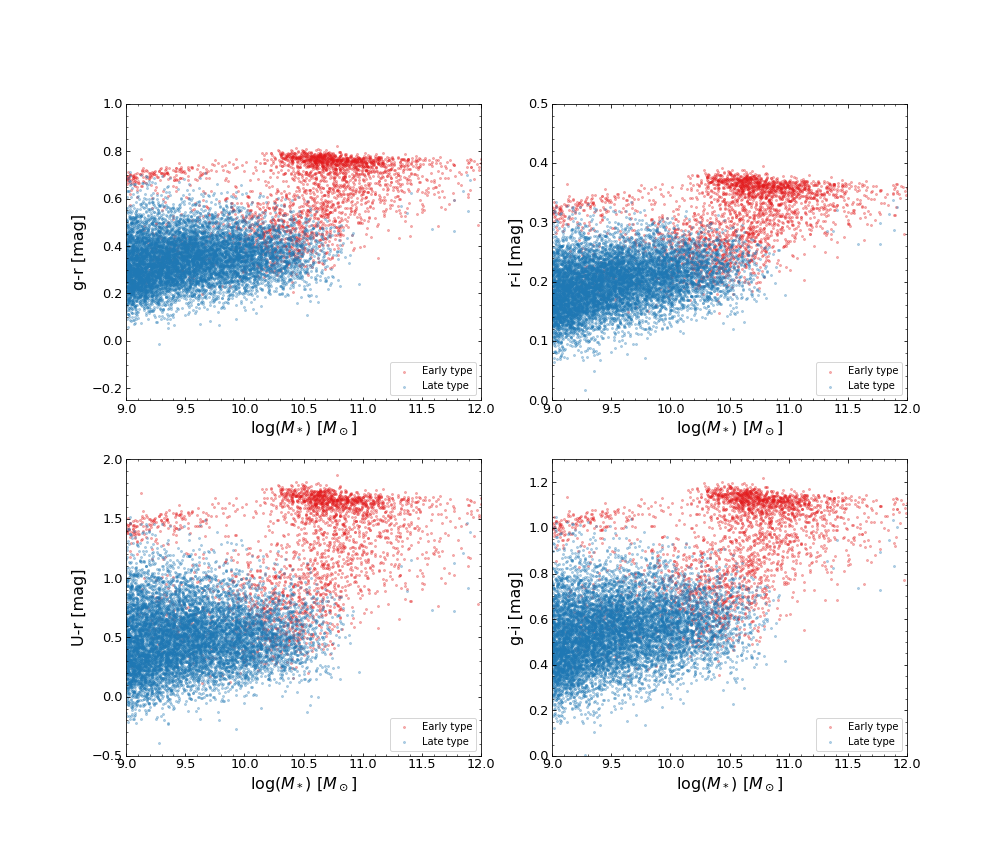
\includegraphics[width=0.9\paperwidth]{images/results_color_magnitude.png}}
    \caption{}
    \label{color_magnitude_res}
\end{figure}

\begin{figure}
    \centering
    \makebox[\textwidth][c]{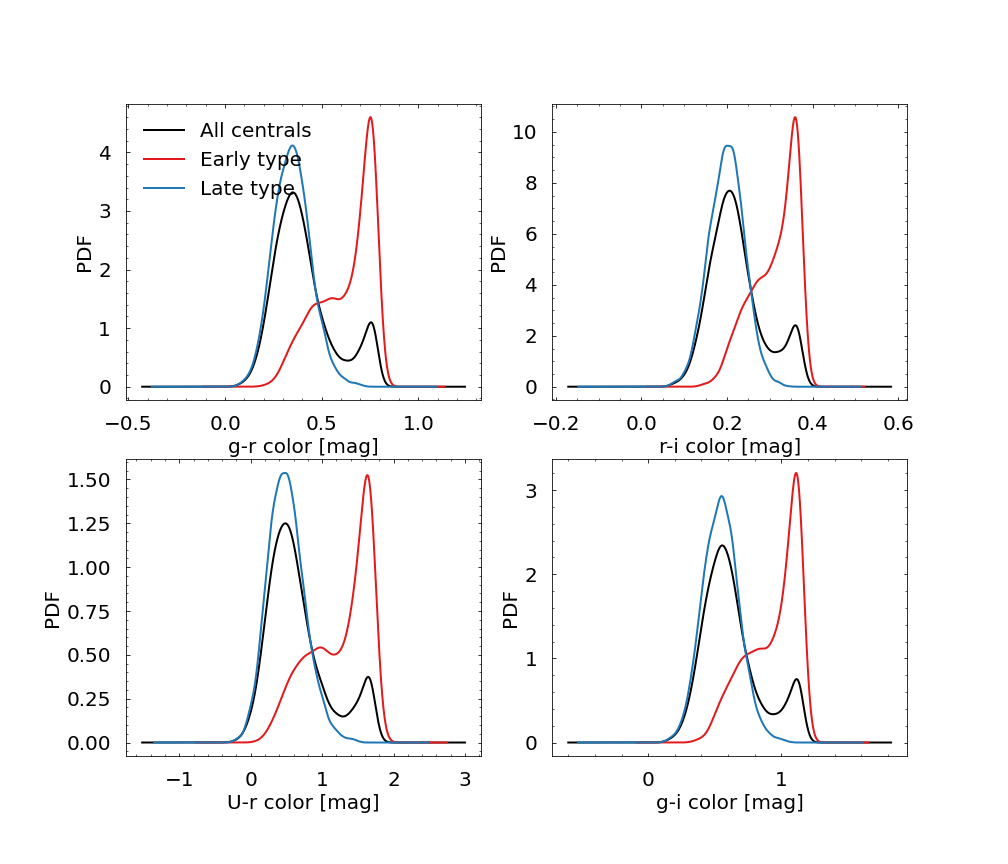
\includegraphics[width=0.9\paperwidth]{images/results_pdf_different_bands.png}}
    \caption{}
    \label{pdf_color_res1}
\end{figure}

\begin{figure}
    \centering
    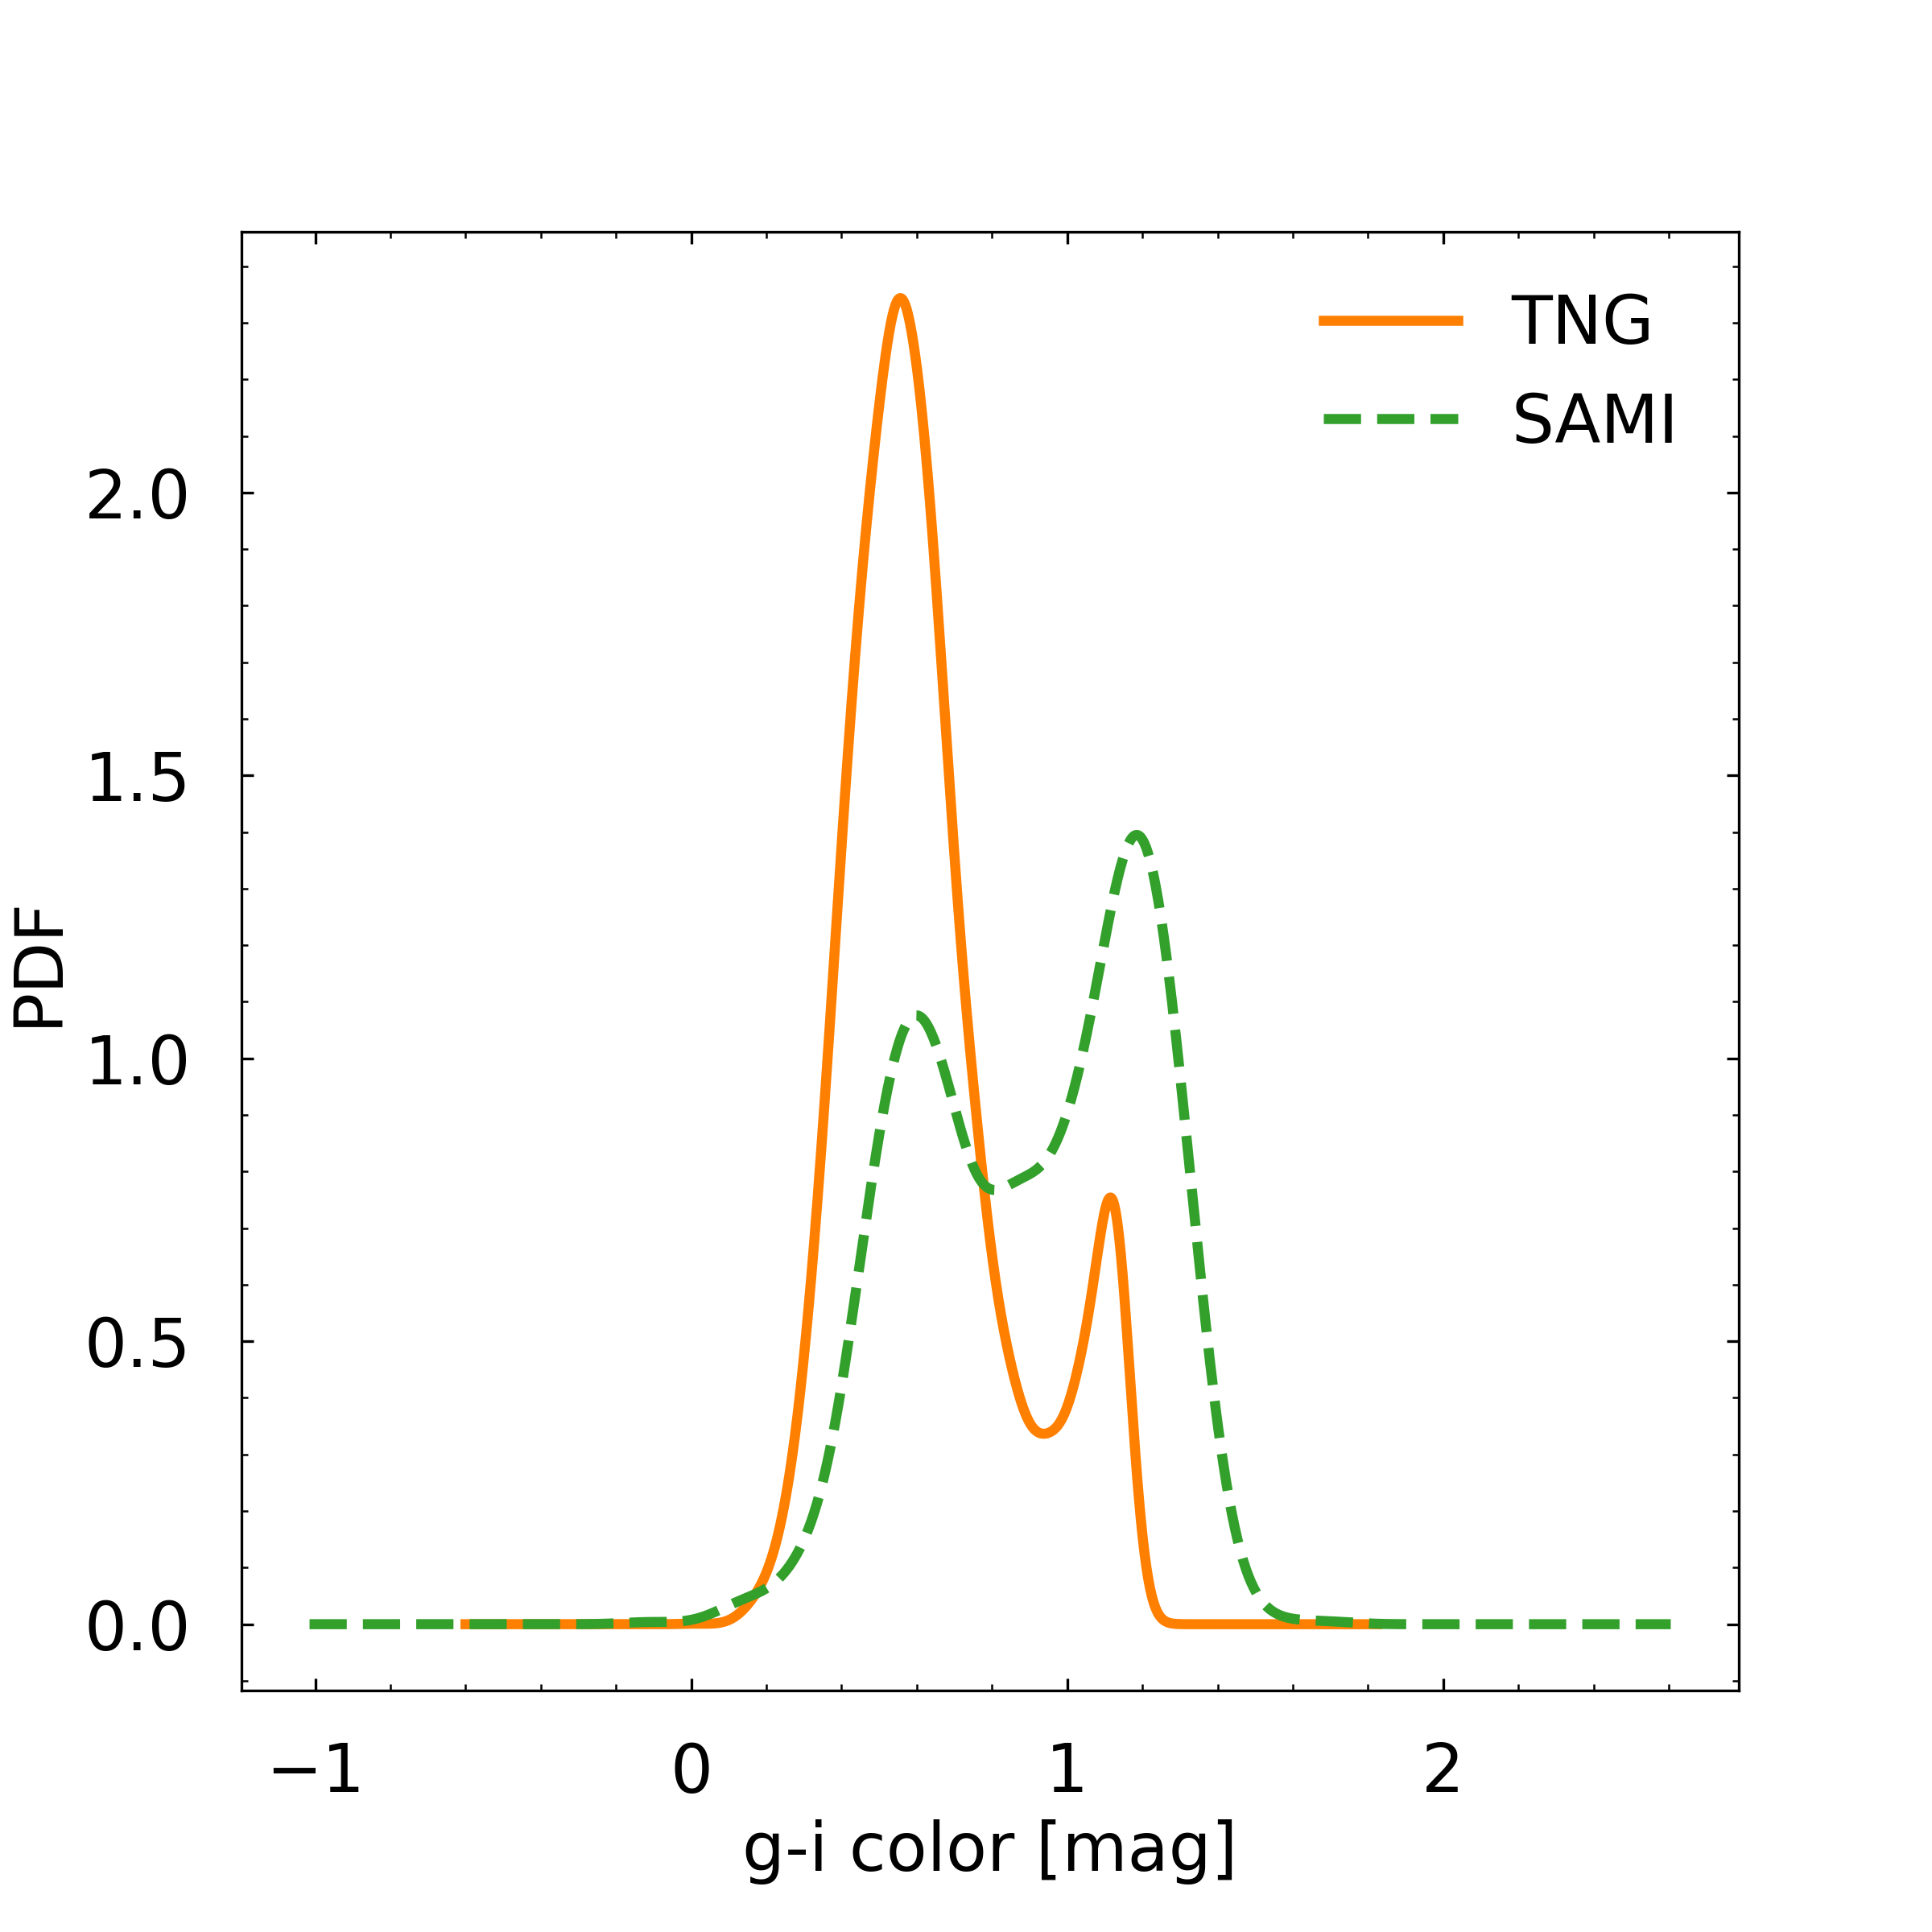
\includegraphics[width=0.9\textwidth]{images/results_pdf_g_i_band.png}
    \caption{}
    \label{pdf_color_res2}
\end{figure}

\subsection{SMBH relations}
In Figure \ref{bh_res} the SMBH-mass and velocity dispersion for TNG100 is shown, along with the best fit functions from \cite{Ferrarese2000} and \cite{Tundo2007}.

\begin{figure}
    \centering
    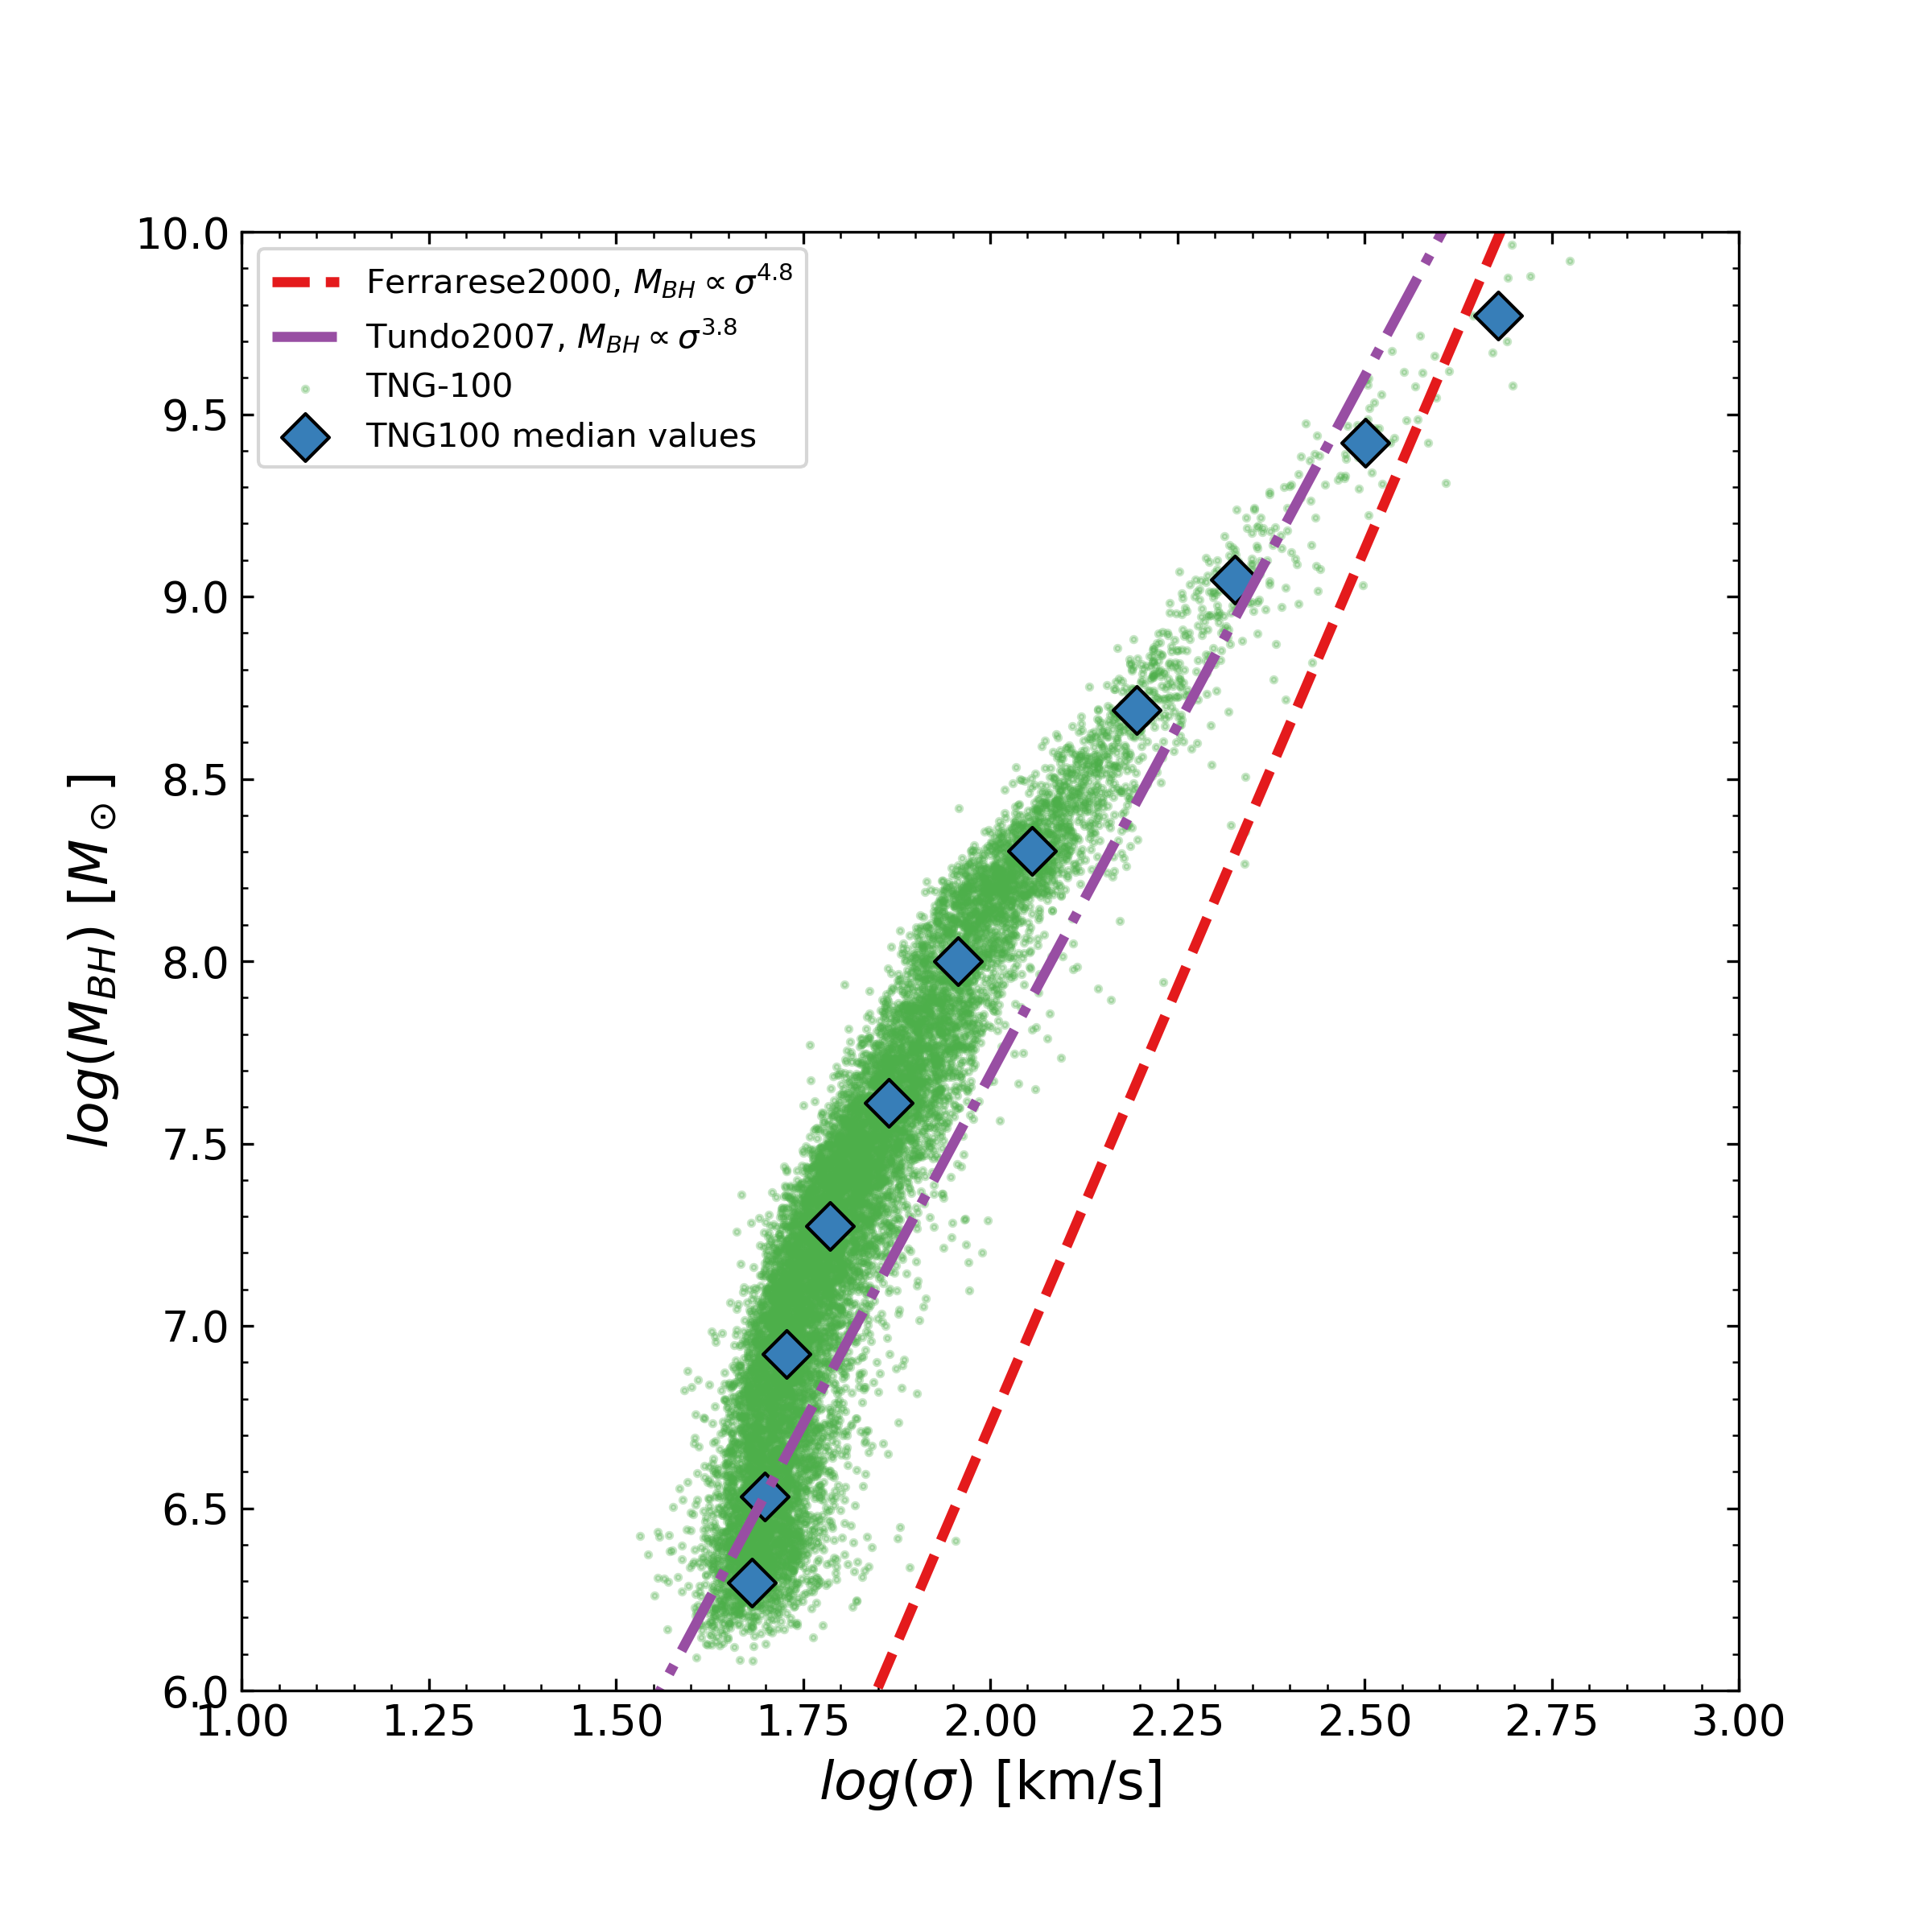
\includegraphics[width=0.9\textwidth]{images/results_mass_BH_sigma.png}
    \caption{}
    \label{bh_res}
\end{figure}